\begin{figure}[!h]
    \centering
    \subfigure[Training set composition per increment. Shaded areas indicate the proportion of replay buffer frames.]{
    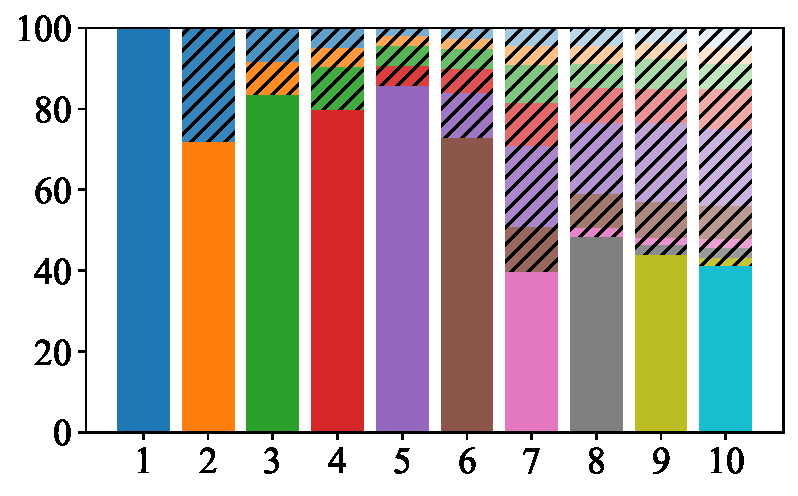
\includegraphics[width=0.43\textwidth]{chapters/ch-conclusion/img/sample.pdf}
    \label{subfig:task_frame_comp}
    }
    \hspace{1mm}
    \subfigure[Per-task accuracy across increments. Each series tracks the accuracy scores for one task.]{%Per-task accuracy. Each series tracks the model's accuracy on a task across increments.]{
    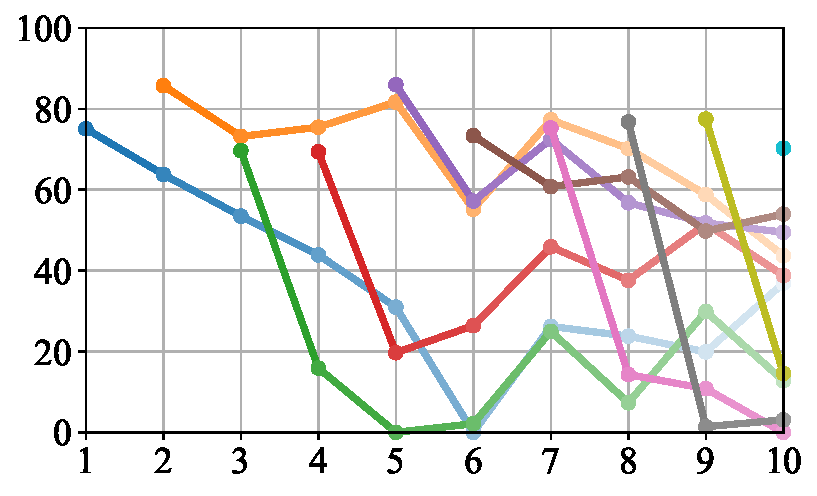
\includegraphics[width=0.43\textwidth]{chapters/ch-conclusion/img/perf.pdf}
    \label{subfig:prevtask_acc}
    }
    \label{fig:imbalance_split1seed42}
    \caption{Effect of task sequence order to training set composition and model performance. %Results shown are from train-test split 1 of Breakfast using task sequence order from seed 42.
    }
\end{figure}